
\documentclass[12pt]{article}
\usepackage[utf8]{inputenc}
\usepackage[T1]{fontenc}
\usepackage{amsmath}

\usepackage{amssymb}
\usepackage{amsmath}
%\usepackage{amsthm}
\usepackage{amsopn}
\usepackage{graphicx}
\usepackage{mathrsfs}

\usepackage{tikz}
\usetikzlibrary{arrows}

%\usepackage{showkeys}



%\setlength{\arraycolsep}{2pt}
%\setlength{\parskip}{.04in}
%\setlength{\footskip}{30pt}

\let\bb\mathbb       % BlackBoardBold (double letters)

\def\1{\mathbf 1}

  \def\AA{{\bb A}}\def\CC{{\bb C}}\def\DD{{\bb D}}\def\EE{{\bb E}}
  \def\GG{{\bb G}}\def\HH{{\bb H}}\def\KK{{\bb K}}\def\LL{{\bb L}}
  \def\MM{{\bb M}}\def\QQ{{\bb Q}}\def\TT{{\bb T}}\def\YY{{\bb Y}}
  \def\PP{{\bb P}}\def\II{{\bb I}}\def\WW{{\bb W}}\def\XX{{\bb X}}
  \def\VV{{\bb V}}\def\SS{{\bb S}}\def\BB{{\bb B}}\def\NN{{\bb N}}
  \def\RR{{\bb R}}\def\ZZ{{\bb Z}}\def\FF{{\bb F}}\def\DD{{\bb D}}
  \def\OO{{\bb O}}\def\JJ{{\bb J}}\def\UU{{\bb U}}

\def\cH{\mathcal H}
\def\cY{\mathcal Y}
\def\cX{\mathcal X}
\def\cA{\mathcal A}
\def\mC{\mathcal C}
\def\Ex{\mathbf E}

\def\bb{\mathbb}
%end of header
\def\hat{\widehat}
\def\bfX{\mathbf X}
\def\bfB{\mathbf B}
\def\bSigma{\boldsymbol\Sigma}
\def\bOmega{\boldsymbol\Omega}
\def\bmu{\boldsymbol\mu}
\def\bnu{\boldsymbol\nu}

\def\bX{\boldsymbol X}
\def\bx{\boldsymbol x}

\def\ci{\perp\!\!\!\perp}

\parskip=3pt
\renewcommand{\baselinestretch}{1.08}


\begin{document}

\section{Pistes de réfléxion Thèse - Janvier 2015}
\subsection{Introduction}

Soient $X_1$,...,$X_n$ un échantillon de n variables aléatoires i.i.d de loi $P^*$, $X_i\in\RR^p$
\\
On suppose que le nombre de clusters (K) est connu, on cherche à approcher $P^*$ par un mélange de Gaussiennes.

$$
P^* = \sum_{j=1}^K \pi_jP_j \qquad avec \qquad \forall i, \quad \pi_i>0 \qquad et \qquad \sum_{j=1}^K\pi_j=1
$$
Où $P_j$ a pour densité la loi normale  $\mathcal N_p(\bmu_j,\bSigma_j)$.
\\

Une approche classique dans le cadre de mélange de gaussien est d'utiliser l'algorithme EM pour estimer les parametres $\Pi,\bmu,\bSigma$. Sans hypothese supplémentaire, la complexite de cette approche rend le calcul impossible quand p devient grand. Une hypothese est de considerer $\bSigma$ diagonale mais ceci revient a considerer que les features sont indépendantes ce qui est un inconvenient.

\subsection{Approche par analyse structurelle de $\Sigma$}

Soient $Y_1$,...,$Y_n$ un échantillon de n variables aléatoires i.i.d de loi $\mathcal N_p(\bmu^*,\bSigma^*)$, $Y_i\in\RR^p$. Supposons p grand. Nous cherchons a estimer $\mu^*$ et $\Sigma^*$.
\\
Nous pouvons estimer la moyenne empirique $\hat{\mu}=\bar{Y_n}$ et donc supposer que $\mu=0$. Pour $\Sigma^*$ ce ci est plus délicat et nous chercherons des hypotheses structurelles sur $\bSigma^{-1}=\bOmega$ la matrice de précison. Notamment en considérant que $\bOmega$ est creuse.
Interpretation: si $\omega_{j,j'}=0$ alors $Y^j \ci Y^{j'}|\{Y^l\backslash (Y^j,Y^{j'})\}$.\\
Nous pouvons considérer le graphe $G=(V,E)$ avec card(V)=p alors,

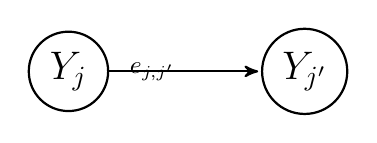
\begin{tikzpicture}[->,>=stealth',shorten >=1pt,auto,node distance=3cm,
  thick,main node/.style={circle,draw,font=\sffamily\Large\bfseries}]

  \node[main node] (1) {$Y_j$};
  \node[main node] (2) [right of=1] {$Y_{j'}$};

\path[every node/.style={font=\sffamily\small}]
   (1) edge node [left] {$e_{j,j'}$} (2);

\end{tikzpicture}
\\
et $e_{j,j'}\in E \iff \omega_{j,j'} \neq 0$

\subsubsection{Graphical Lasso}
On veut le maximum de vraissemblance pénalisé par la norme $L_1$.

$$
\hat\bOmega \in \text{arg}\min_{\bOmega\geq0\\}
\Big\{\log(\det\Omega)+\frac12 tr (\Omega S_n)+\lambda\parallel\Omega\parallel_1 \}
$$
\\
avec $S_n=\frac1n\sum_{i=1}^nY_iY_i^T$ la matrice de covariance et
$\|\bOmega\|_1= \sum_{j,j':j\not=j'}|\omega_{j,j'}|$
Ceci est un probleme d'optimisation convexe, (problème d'optimisation SDP)


\subsubsection{Column-wize Lasso}

(Théoreme)
Si $Y\sim\mathcal N_p(0,(\Omega^*)^{-1})$, alors $Y_j=\sum_{j=1,j\not=j'}^p(PROUT)$

\end{document}
